\documentclass[10pt]{beamer}

\usetheme[progressbar=frametitle]{metropolis}
\usepackage{appendixnumberbeamer}
\usepackage{amssymb}
\usepackage{booktabs}
\usepackage[scale=2]{ccicons}
\usepackage{tikz}
\usepackage{pgfplots}
\usepgfplotslibrary{dateplot}
\usepackage{wrapfig}
\usepackage{xspace}
\newcommand{\themename}{\textbf{\textsc{metropolis}}\xspace}

\usepackage{graphicx}

\usepackage{subcaption}

\usepackage[export]{adjustbox}
\title{EE5327 : Optimization}
% \date{\today}
\date{}
\author{Harsh Raj - MA17BTECH11003 \newline Aravind Reddy K V - MA17BTECH11010}
\institute{Mathematics and Computing, IIT-Hyderabad}
% \titlegraphic{\hfill\includegraphics[height=1.5cm]{logo.pdf}}
\begin{document}
\maketitle
%begin{frame}{Table of contents}
%  \setbeamertemplate{section in toc}[sections numbered]
%  \tableofcontents[hideallsubsections]
%\end{frame}

%\section{Recommender Systems Strategies}

%\begin{frame}[fragile]{Recommender Systems Strategies}
%   \begin{itemize}
%    \item Electronic retailers and content providers offer a huge selection of products to meet a variety of special needs and tastes.
%    \item Matching consumers with the most appropriate products is key to enhancing user satisfaction and loyalty.
%    \item Therefore, more retailers and e-commerce leaders like Amazon and Netflix have become interested in recommender systems, which analyze patterns of %user interest in products to provide personalized recommendations that suit a user's taste.
%    \end{itemize}
%\end{frame}
\section{Recommender Systems Strategies}
\begin{frame}[fragile]{Recommender Systems Strategies}
\begin{center}
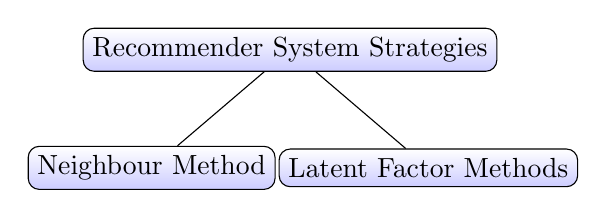
\begin{tikzpicture}[sibling distance=10em,
  every node/.style = {shape=rectangle, rounded corners,
    draw, align=center,
    top color=white, bottom color=blue!20}]]
  \node {Recommender System Strategies}
    child { node {Neighbour Method} }
    child { node {Latent Factor Methods} };
\end{tikzpicture}
\end{center}
\\
%\begin{itemize}

%\item The \textbf{content filtering} approach creates a profile for each user or product to characterize its nature.
%\item The profiles allow programs to associate users with matching products. 
%\item Content-based strategies require gathering external information that might not be available or easy to collect.
%\end{itemize}
%\end{frame}

%\begin{frame}[fragile]{Collaborative Filtering}
% \textbf{Collaborative filtering} relies only on past user behavior—for example, previous transactions or product ratings—without requiring the creation of explicit profiles.
% \\
% \vspace{3mm}
% The two primary areas of collaborative filtering are the \textbf{neighborhood methods} and \textbf{latent factor models}.
 \begin{center}
 \graphicspath{ {./images/} }
 \includegraphics [scale=0.2] {3}
 \end{center}
\end{frame}

\begin{frame}[fragile]{Neighbourhood Method}

 This method involves finding $K$-nearest neighbours (\textbf{K-NN} algorithm and it's variants).\\
 \vspace{3mm}
 \begin{center}
 \graphicspath{ {./images/} }
 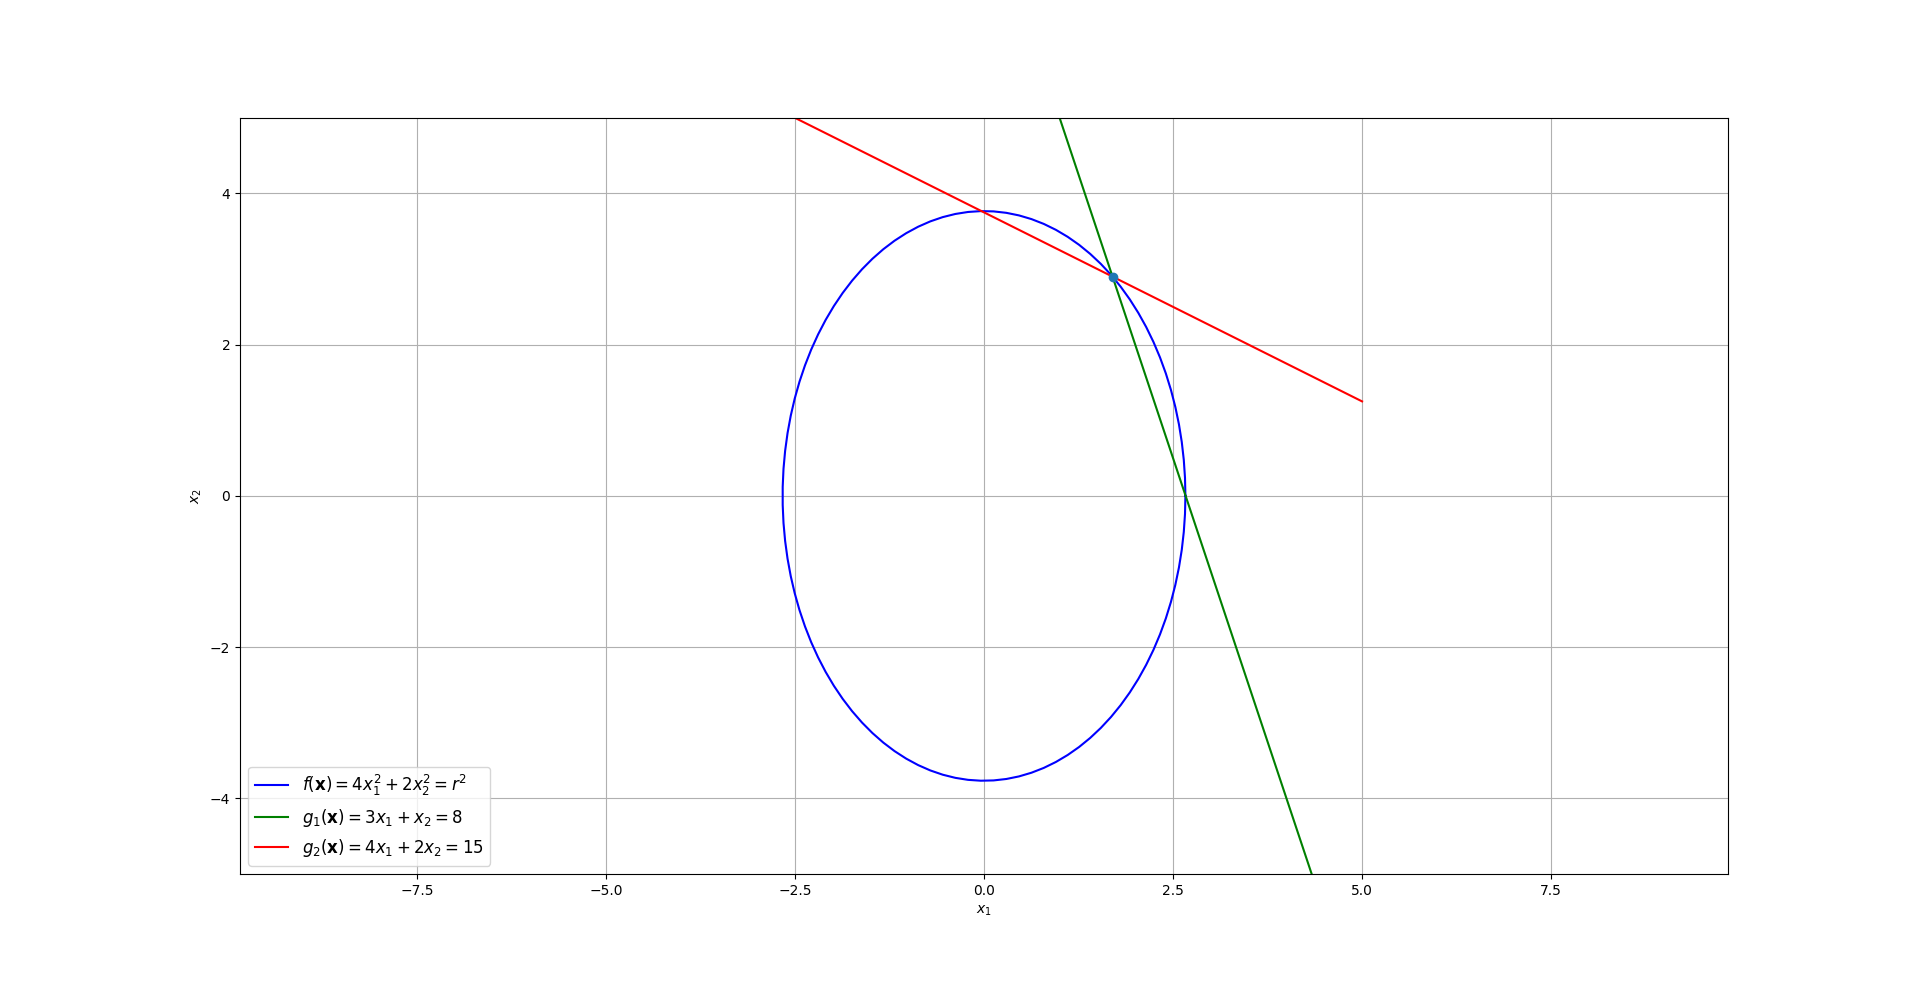
\includegraphics [scale=0.2] {1}
 \end{center}
  Why is this method very slow and also not accurate always?
 \newline
  - If predicting among all possibilities, requires \textbf{O(n)} iterations for each prediction.
  \newline 
  - Only predicts within predetermined cluster if time reduced to \textbf{O(1)}.
  \newline
  - Cannot Incorporate Item/User based Bias
\end{frame}

\begin{frame}[fragile]{Latent Factor Models}
 \textbf{Latent factor models} try to explain the ratings by characterizing both items and users on factors inferred from the ratings patterns.
 \begin{center}
 \graphicspath{ {./images/} }
 \includegraphics [scale=0.2] {2}
 \end{center}
User's predicted relative rating for a movie =
\newline \textbf{Dot product} of the movie's and user's location vectors on \text\textbf{Latent Space}. 
\end{frame}

%\begin{frame}[fragile]{Matrix Factorization Meth%ods}
%  \begin{item%ize}
%      \item Some of the most successful realizations of latent factor models are based on \textbf{matrix factorizati%on}.
%      \item In its basic form, matrix factorization characterizes both items and users by vectors of factors inferred from item rating patte%rns.
%  \end{item%ize}
%   Recommender systems rely on different types of \textbf{input data}, which are often placed in a matrix with one dimension representing users and the other %dimension representing items of interes%t.\\
%   \vspace{%3mm}
%   The input form could be either \textbf{explicit feedback} or \textbf{implicit feedb%ack}
%\end{frame}


\begin{frame}[fragile]{Input Data}
 \begin{enumerate}
   \item \textbf{\textit{Explicit Feedback}}
   \vspace{3mm}
   \begin{itemize}
     \item Explicit input by users regarding their interest in products.
     \vspace{3mm}
     \item Comprises a \textbf{Sparse Matrix}, since any single user is likely to have rated only a small percentage of possible i
      \vspace{3mm}
     \item \textbf{High confidence} on this data.
   \end{itemize}
   \vspace{3mm}
   \item \textbf{\textit{Implicit Feedback}}
   \vspace{3mm}
   \begin{itemize}
       \item Observing user behavior, including purchase history, browsing history, search patterns etc.
       \vspace{3mm}
       \item Denotes the presence or absence of an event, so it is typically represented by a \textbf{Dense Matrix}
       \vspace{3mm}
     \item \textbf{Low confidence} on this data.
   \end{itemize}
\end{enumerate}
\end{frame}

\begin{frame}[fragile]{Matrix Factorization Model}
Matrix factorization models map both users and items to a joint \textbf{Latent Factor Space} of dimensionality \boldsymbol{f}.\\
\vspace{3mm}
Each item \boldsymbol{i} is associated with a vector \boldsymbol{q_i} $\in \mathbb{R}^{f} $, quantizing the amount of each attribute present in item {i}.
\newline Each user \boldsymbol{u} is associated with a vector \boldsymbol{p_u} $\in \mathbb{R}^{f}$, quantizing the weightage of each attribute in the user's final decision.\\
\vspace{3mm}
The resulting dot product, \boldsymbol{q_i^{T} p_u}, captures the user \boldsymbol{u}’s overall interest in the item \boldsymbol{i}.\\
\vspace{3mm}
This approximates user \boldsymbol{u}'s estimated rating of item \boldsymbol{i}, denoted by \boldsymbol{\hat{r}_{ui}}:
\begin{equation}
    \boldsymbol{\hat{r}_{ui}=q_{i}^{T}p_{u}}.
\end{equation}
\end{frame}

\begin{frame}{Example}

For 5 movies, 7 latent attributes, we get : 
\newline \newline
\begin{bmatrix}
q_{11} &  q_{12}&  q_{13}&  q_{14}&  q_{15}&  q_{16}&  q_{17}& \\ 
q_{21} &  q_{22}&  q_{23}&  q_{24}&  q_{25}&  q_{26}&  q_{27}& \\ 
q_{31} &  q_{32}&  q_{33}&  q_{34}&  q_{35}&  q_{36}&  q_{37}& \\ 
q_{41} &  q_{42}&  q_{43}&  q_{44}&  q_{45}&  q_{46}&  q_{47}& \\ 
q_{51} &  q_{52}&  q_{53}&  q_{54}&  q_{55}&  q_{56}&  q_{57}& \\ 
\end{bmatrix}
\begin{bmatrix}
p_{1} &\\ 
p_{2} &\\ 
p_{3} &\\ 
p_{4} &\\ 
p_{5} &\\ 
p_{6} &\\ 
p_{7} &\\ 
\end{bmatrix}
=
\begin{bmatrix}
\hat{r}_{1} &\\ 
\hat{r}_{2} &\\ 
\hat{r}_{3} &\\ 
\hat{r}_{4} &\\ 
\hat{r}_{5} &\\ 
\end{bmatrix}
\end{frame}


\begin{frame}{Optimization  Problem}
    %Minimizes the regularized squared error on the set of known ratings
     Introduce Regularization Parameter to avoid overfitting. 
     To learn the factor vectors \boldsymbol{p_u} and \boldsymbol{q_i}, the system minimizes the regularized squared error on the set of known ratings:
    \begin{center}
    {\min\limits_{q^{\star}, p^{\star}}$\sum\limits_{(u,i)\in \kappa}(r_{ui}-q_{i}^{T} p_{u})^{2}+\lambda(\Vert q_{i}\Vert^{2}+\Vert p_{u}\Vert^{2})$}
\end{center}

The constant $\lambda$ controls the extent of regularization, by keeping each attribute close to zero. $\lambda$ is determined by cross-validation. 
\end{frame}

\begin{frame}{Learning Algorithm : SGD}
    One option is to use Stochastic Gradient Descent Algorithm, i.e.,
    $e_{ui} = r_{ui}- {q_i}^T p_u$
    \newline
    $q_i \longleftarrow q_i + \gamma(e_{ui}p_u - \lambda q_i)$
    \newline
    $p_u \longleftarrow p_u + \gamma(e_{ui}q_i - \lambda p_u)$
    \newline \newline
    \textbf{Problems :}
    \newline \newline
    - Requires $\textbf{O(n)}$ operations for each iteration. 
    \newline. \hspace{2mm} Feasible only for $\textbf{Sparse Matrix}$. 
    \newline. \hspace{3mm}$\implies$ Cannot Use $\textbf{Implicit Feedback}$ Data.
    \newline
    - All operations must be performed in serial order. 
\end{frame}

\begin{frame}{Learning Algorithm : ALS}
    \textbf{Alternating Least Squares:}
    \newline \newline
    As both \boldsymbol{p_u} and \boldsymbol{q_i} are unknown, the objective is not Convex. 
        \begin{equation}
        \sum\limits_{(u,i)\in \kappa}(r_{ui}-q_{i}^{T} p_{u})^{2}+\lambda(\Vert q_{i}\Vert^{2}+\Vert p_{u}\Vert^{2})
        \end{equation}
    \newline
    If we fix one of the unknowns, the optimization problem becomes Quadratic Convex (QCP) and can be solved optimally.
    \newline \newline
    ALS technique rotates between fixing \boldsymbol{q_i}’s and \boldsymbol{p_u}’s. 
    \newline When all \boldsymbol{p_u}’s are fixed, the system recomputes the \boldsymbol{q_i}’s by Directly solving a least-squares problem, and vice-versa. 
    \newline Each step decreases objective function until convergence.
\end{frame}

\begin{frame}{Learning Algorithm : ALS}
\textbf{Repeat Until Convergence: }
\begin{center}
    {(i) \min\limits_{q^{\star}}$\sum\limits_{(u,i)\in \kappa}(r_{ui}-q_{i}^{T} p_{u})^{2}+\lambda(\Vert q_{i}\Vert^{2}+\Vert p_{u}\Vert^{2})$}
\end{center}
\begin{center}
    {(ii) \min\limits_{p^{\star}}$\sum\limits_{(u,i)\in \kappa}(r_{ui}-q_{i}^{T} p_{u})^{2}+\lambda(\Vert q_{i}\Vert^{2}+\Vert p_{u}\Vert^{2})$}
\end{center}
    \textbf{Advantages :}
    \newline \newline
    - Feasible for $\textbf{Dense Matrix}$. 
    \newline. \hspace{2mm}$\implies$ Can Use $\textbf{Implicit Feedback}$ Data.
    \newline
    - All \boldsymbol{p_i} are computed independent of other factors (same for all \boldsymbol{q_i}).
    \newline. \hspace{2mm}$\implies$ Parallelization can be done here. 
\end{frame}

\begin{frame}{Adding Biases and Confidence}

Incorporate \textbf{Bias} in this model - 
\newline \newline
(i) \boldsymbol{\mu} :  Shifts the Prediction Mean from 0 to \boldsymbol{\mu} 
\newline . \hspace{7mm} where \boldsymbol{\mu}= Overall Average Rating
\newline
(ii) \boldsymbol{b_i} : Item Based Bias
\newline . \hspace{7mm} where \boldsymbol{b_i}= Average Rating of Item i -  Overall Average Rating
\newline
(iii) \boldsymbol{b_u} : User Based Bias
\newline . \hspace{7mm} where \boldsymbol{b_u}= Average Rating by User u -  Overall Average Rating
\newline \newline

Incorporate \textbf{Confidence} in this model - 
\newline \newline
(iv) \boldsymbol{c_{ui}} :  Confidence in observing \boldsymbol{r_{ui}} 

%(iv) $\boldsymbol{{\mid N(u) \mid}}^{-0.5}$ $(\sum\limits_{i \in N(u)}\boldsymbol{x_i} )$: Normalized Implicit Feedback
%\vspace{2mm}
%\newline . \hspace{7mm} where \boldsymbol{\mid N(u)\mid}= Items with Implicit Feedback from User u
%\newline . \hspace{7mm} and \boldsymbol{x_i} = Implicit Feedback Vector for i $\in \boldsymbol{N(u)}$
%\newline
\end{frame}


\begin{frame}{Final Recommender}
    \newline Final Prediction is : \newline
 $   \boldsymbol{\hat{r}_{ui}}=c_{ui}(\mu + b_u + b_i + {p_u}^T q_i) $
 \newline \newline
 Final form of Recommender: 
    \begin{center}
    {\min\limits_{q^{\star}, p^{\star},b^{\star}}$\sum\limits_{(u,i)}c_{ui}(r_{ui}- \mu -b_u -b_i - q_{i}^{T} p_{u})^{2}+\lambda(\Vert q_{i}\Vert^{2}+\Vert p_{u}\Vert^{2} +\Vert b_{u}\Vert^{2} +\Vert b_{i}\Vert^{2} )$
    }
\end{center}
subject to : $c_{ui} \geqslant 0 $ $\forall (u,i) $
\newline. \hspace{1.53cm} $ \lambda \geqslant 0 $



\end{frame}

\begin{frame}{Proof of Convexity}
\textbf{Claim:} For a fixed $p_u$, \newline $\sum\limits_{(u,i)}c_{ui}(r_{ui}- \mu -b_u -b_i - q_{i}^{T} p_{u})^{2}+\lambda(\Vert q_{i}\Vert^{2}+\Vert p_{u}\Vert^{2} +\Vert b_{u}\Vert^{2} +\Vert b_{i}\Vert^{2} )$ \newline
is convex in q_{i}. 
\newline \newline \textbf{Proof:}\newline
i) $(r_{ui}- \mu -b_u -b_i - q_{i}^{T} p_{u})$ is affine in q_{i}
\newline
ii) $(r_{ui}- \mu -b_u -b_i - q_{i}^{T} p_{u})^{2}$ is convex in $q_{i}$ as it is square of affine function
\newline
iii) $\lambda(\Vert q_{i}\Vert^{2} )$ is convex in $q_{i}$ because it is a norm.
\newline
iv) As sum of convex functions is convex, adding ii) and ii), we get, \newline $\sum\limits_{(u,i)}c_{ui}(r_{ui}- \mu -b_u -b_i - q_{i}^{T} p_{u})^{2}+\lambda(\Vert q_{i}\Vert^{2}+\Vert p_{u}\Vert^{2} +\Vert b_{u}\Vert^{2} +\Vert b_{i}\Vert^{2} )$ is convex. \newline(Proved)
\end{frame}

\begin{frame}{Accuracy Improvement}

Original Netflix system : \newline RMSE = 0.9514
\newline \newline
Plain Matrix Factorization Model : \newline RMSE = 0.9025
\newline \newline
Included User and Item Biases : \newline RMSE = 0.9000
\newline \newline
Included Implicit Feedback and Confidence Parameter : \newline RMSE = 0.8925

\end{frame}

\end{document}
